\documentclass[9pt]{beamer}

\usepackage{hyperref}
\usepackage[utf8]{inputenc} 
\usepackage[english]{babel}
\usepackage{fancyhdr}
\usepackage{amsmath,amssymb}
\usepackage{array}
%\usepackage{style}
\usepackage{amsthm}
\usepackage[toc,page]{appendix}
\usepackage{color}
\usepackage{graphicx}
\usepackage{frontespizio}
\usepackage{faktor}
\usepackage{hyperref}
\usepackage{frontespizio}
\usepackage{pdfpages}
\usepackage{listings}
\usepackage{import}
\usetheme{JuanLesPins}
\usefonttheme{serif}
\newcommand{\sg} {
  \boldsymbol{\mu}}
 \newcommand{\Nd}{N_{\delta}}
\newcommand{\Nc}{N}
\newcommand{\Bc}{\mathcal{B}}
\newcommand{\bu}{\textbf{u}}
\newcommand{\bv}{\textbf{v}}
\usepackage{verbatim}
\usepackage{afterpage}
\newcommand{\og}{\omega}


\title{Metrics for Binary Classification}
\author{Julien Genovese}
\institute{Machine Learning Together Milan}
\date{14th December 2020}

\begin{filecontents}{abc.bib}
@article{bilson1978rational,
title={Rational expectations and the exchange rate},
author={Bilson, John FO},
journal={The economics of exchange rates: Selected studies},
pages={75--96},
year={1978}
}
\end{filecontents}


\begin{document}
\begin{frame}
\maketitle
\begin{figure}[ht]

\includegraphics[scale=0.25]{images/MLTM.jpeg}
\quad
\end{figure}
\end{frame}

\begin{frame}
\frametitle{Table of Contents}
\tableofcontents
\end{frame}

\section{Classification problem basics}
\begin{frame}
\frametitle{What is classification?}
\begin{itemize}
\item \textbf{Classification is the problem of dividing an observation in a certain category according to its properties}.
\item Some examples: Is this a triangle, a rectangle or a circle? What kind of character we have?
\vspace{10mm}
\begin{figure}[ht]
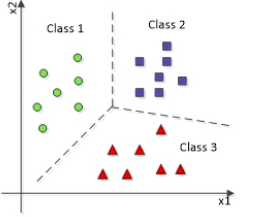
\includegraphics[scale=0.50]{images/classificationintroduction.png}
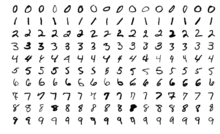
\includegraphics[scale=0.50]{images/Mnist.png}
\caption{Two examples of classification}
\end{figure}
\end{itemize}
\end{frame}

\begin{frame}
\frametitle{Types of classification problems}
\begin{itemize}
\item We can have two main types of classification: \textbf{binary} and \textbf{multiclass}.
\item The classification can be \textbf{balanced} and \textbf{imbalanced}:
\begin{itemize}
\item Balanced: in this case all the classes have similar frequencies.
\item Imbalanced: some classes are more frequent that other ones.\\ Example: classification between rare and common events.
\vspace{5mm}
\begin{figure}[ht]
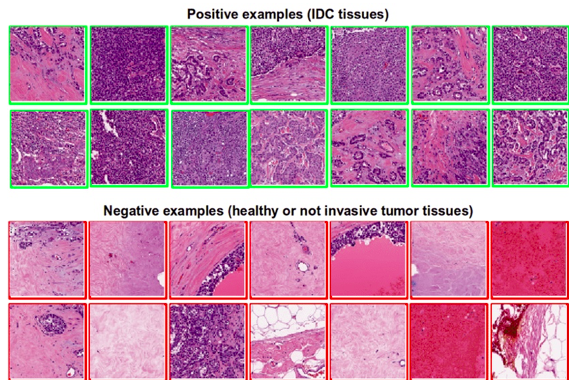
\includegraphics[scale=0.30]{images/tumor.png}
\caption{Disease vs not disease}
\end{figure}
\end{itemize}
\end{itemize}
\end{frame}

\begin{frame}
\frametitle{Mathematical model for classification}
\begin{itemize}
\item A classifier (algorithm to classify) gives us a \textbf{probability} to belong to a class and with a \textbf{threshold} that we decide we obtain the \textbf{label} associated to a class.
\item Classification is a \textbf{supervised machine learning problem}, where we have an input of features $X$, and an output $Y$, and we want to learn the relationship $f$ between them.
\item The mathematical model is in the general form of:
$$
p = f(X) + \varepsilon
$$
where $p$ is the \textbf{estimated probability} to belong to a certain class $\in Y$, $X$ the \textbf{input}, $\varepsilon$ an \textbf{error term} related to the stochasticity, $f$ is the \textbf{relationship} between the input and the output and this is what the algorithm want to learn.
\end{itemize}
\end{frame}

\begin{frame}
\frametitle{Binary classification}
\begin{itemize}
\item In a binary problem we select one of the two class, that we call the "positive class" and $p$ is the probability to belong to this class, $1-p$ the probability for the other class, the "negative class".
\item Example: the logistic regression is in the implicit form of:
$$
\log(\dfrac{p}{1-p}) = \beta_0 + \beta_1 x_1 + \beta_2 x_2
$$
and if we explicit $p$:
$$
p = P(Y = 1) = \dfrac{1}{1+ e^{-(\beta_0 + \beta_1 x_1 + \beta_2 x_2)}}
$$
\end{itemize}
\end{frame}


\section{Calibration plot}
\begin{frame}
\frametitle{Calibration of the Probabilities}
\begin{itemize}
\item We desire that the estimated class probabilities are reflective of the true underlying probability of the sample, that is, \textbf{well-calibrated}.
\item Example: if we predict that a mail is spam with a 0.2 probability, we want that if we take 5 similar mails, only one of them is spam.
\item To do it we use a \textbf{calibration plot}.
\item The next definition is \textbf{only for balanced problems}.
\end{itemize}
\end{frame}

\begin{frame}
\frametitle{How to do a Calibration Plot}
\begin{itemize}
\item First fix a set of bins like $[0, 10\%], (10\%, 20\%], ..., (90\%, 100\%]$.
\item In each bin put all the observations you have according to the probability. Example: an observation with $0.15$ probability will be assegnated to the bin $(10\%, 20\%]$.
\item Compute the number of events with the class associated to the probability $p$, divide it by the number of observation in the bin: this is the \textbf{observed event rate}.
\item If the probability reflects the true underlying probability of the sample, the observed event rate must stay on the diagonal. In this case we say that the probabilities are \textbf{well-calibrated}.
\end{itemize}
\end{frame}

\begin{frame}
\frametitle{An example of a Calibration Plot}
\begin{itemize}
\item In the figure we have the results of two model predictions. We see both an example of well-calibrated and not-well calibrated plot. 
\begin{figure}[ht]
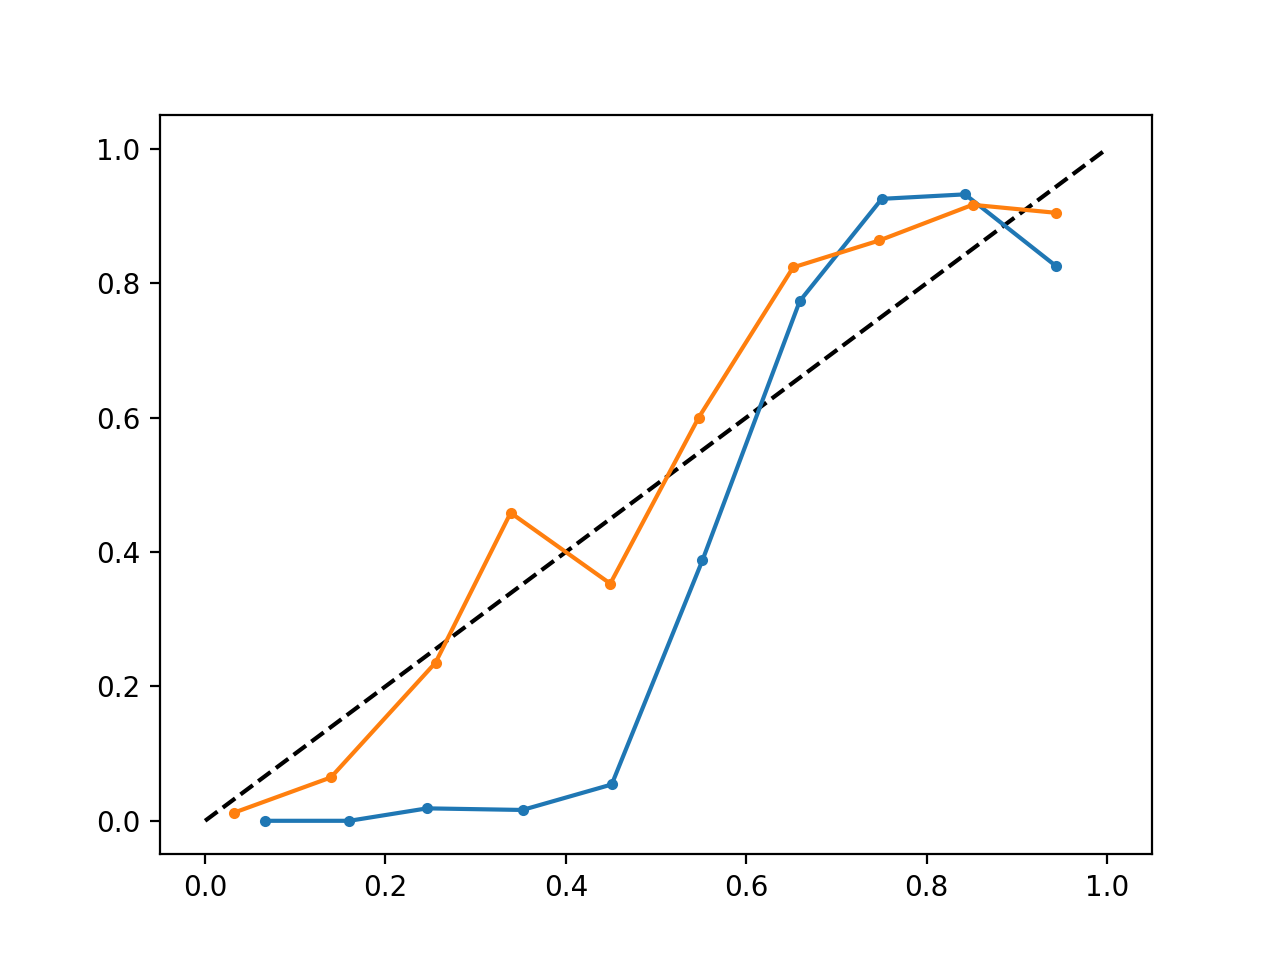
\includegraphics[scale=0.25]{images/Calibrated-and-Uncalibrated.png}
\caption{An example of well-calibrated in orange and not-well calibrated plot in blue}
\end{figure}
\end{itemize}
\end{frame}

\section{Robustness of class Probability}
\begin{frame}
\frametitle{Presenting Class Probabilities}
\begin{itemize}
\item For a binary classification problem we have a good tool to understand the robustness of a model, i.e. if our model is very sure of its prediction.
\item An easy tool is to plot an histogram of the probabilities for each class.
\item We want the probabilities for the positive class distributed on the right and the probabilities for the negative one on the left.
\item In this way we have a tool to understand how the model is sure of what is saying.
\end{itemize}
\end{frame}
\begin{frame}
\frametitle{Two examples of Class Probabilities}
\begin{figure}[ht]
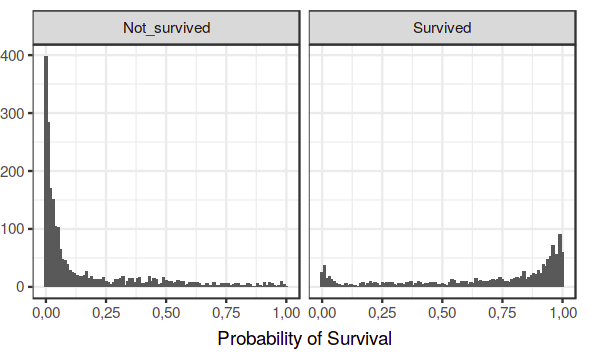
\includegraphics[scale=0.30]{images/goodexample.png}
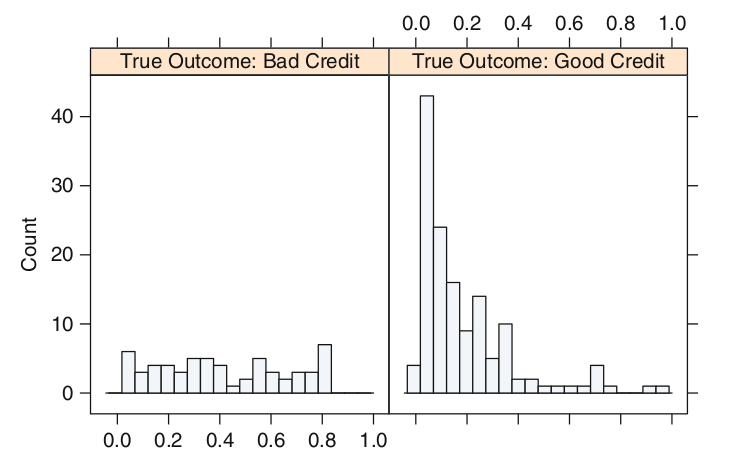
\includegraphics[scale=0.25]{images/robustnessprob.png}
\caption{A robust classifier on the left and a not-robust one on the right}
\end{figure}
\end{frame}
\section{Metrics for classification}
\begin{frame}
\frametitle{Confusion matrix}
\begin{itemize}
\item To understand the validity of a classifier we want to understand how many events we have right predicted, how many mistakes have been done, and which ones.
\item A classical tool is the \textbf{confusion matrix}.
\begin{figure}[ht]
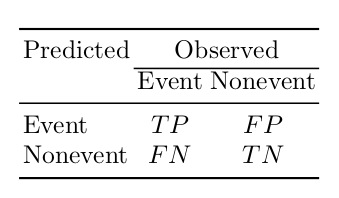
\includegraphics[scale=0.25]{images/confusionmatrix.png}
\caption{A general confusion matrix}

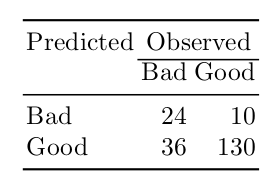
\includegraphics[scale=0.30]{images/exampleConfusionMatrix.png}
\caption{An example of confusion matrix}
\end{figure}
\item With this matrix we can create different metrics.
\end{itemize}

\end{frame}


\begin{frame}
\frametitle{Accuracy rate}
\begin{itemize}
\item The accuracy rate is defined as:
$$
\dfrac{\mbox{True predictions}}{\mbox{All the events}}
$$
that we translate as:
$$\dfrac{TP + TN}{TP + TN + FP + FN}.$$
\item This metric doesn't take into account:
\begin{itemize}
\item \textbf{the errors that have been made}.
\item \textbf{the frequencies of each class}.
\end{itemize}
Ex: in an imbalanced problem the positive class could be $99\%$. In this case an algorithm that predict all the events as the most frequent class has an accuracy of $0.99$ that seems good but it's not.
\end{itemize}
\end{frame}

\begin{frame}
\frametitle{An example of accuracy computation}
Let's suppose we have a confusion matrix like that:
\begin{table}
\begin{tabular}{l | c | c | c | c }
Predicted | Reference & Positive & Negative \\
\hline \hline
Positive + & 300 & 60 \\ 
Negative - & 200 & 855 \\
\end{tabular}
\end{table}
In this case the accuracy is:
$$
\dfrac{300 + 855}{300 + 855 + 200 +60}\cdot 100 = 82 \% 
$$
\end{frame}

\begin{frame}
\frametitle{Sensitivity (Recall) and Specificity}
\begin{itemize}
\item $ \mbox{\textbf{Sensitivity}} = \dfrac{\# \mbox{positive samples and predicted to be positives}}{\# \mbox{Positive samples}} = \dfrac{\mbox{TP}}{\mbox{TP + FN}}$.\\
\vspace{2mm}
This is the ability to \textbf{detect positive samples}.
\item $\mbox{\textbf{Specificity}} = \dfrac{\# \mbox{negative samples and predicted as negatives}}{\# \mbox{Negative samples}} = \dfrac{\mbox{TN}}{\mbox{TN+FP}}$.\\
\vspace{2mm}
This is the ability to \textbf{detect negative samples}.
\end{itemize}
\end{frame}

\begin{frame}
\frametitle{An example of Sensitivy and Specificity computation}
Let's suppose we have a confusion matrix like that:
\begin{table}
\begin{tabular}{l | c | c | c | c }
Predicted | Reference & Positive & Negative \\
\hline \hline
Positive + & 300 & 60 \\ 
Negative - & 200 & 855 \\
\end{tabular}
\end{table}
In this case the sensitivity is:
$$
\dfrac{300}{300 + 200}\cdot 100 = 60 \% 
$$
and the specificity:
$$
\dfrac{855}{855 + 60}\cdot 100 = 93 \% 
$$
\end{frame}

\begin{frame}
\frametitle{Probabilistic interpretation}
\begin{itemize}
\item Sensitivity and specificity are two conditional probabilities.
\item We use a medical explaination:
\begin{itemize}
\item Sensitivity is defined as the probability of a positive test result given the presence of disease, written as:
$$ P(\mbox{positive test} | \mbox{disease present}) .$$
\item Specificity is defined as the probability of a negative test result given the absence of disease, written as:
$$ P(\mbox{negative test} | \mbox{disease absent}) .$$
\end{itemize} 
\item These quantities doesn't depend on prevalence, that is the frequence of the positive class definied as:
$$
\mbox{Prevalence} =\dfrac{\# \mbox{Positive samples}}{\# \mbox{All samples}} =\dfrac{TP + FN}{ TP+FN+FP+TN}
$$
because these probabilities only depends on the test.
\end{itemize}
\end{frame}

\begin{frame}
\frametitle{Sensitivity-Specificity trade-off}
\begin{itemize}
\item We know that changing the threshold we change the labels and so specificity and sensitivity.
\item \textbf{Decreasing the threshold} we increase the number of true positives but the number of real positives is the same. So the \textbf{sensitivity increases}. 
\item \textbf{Decreasing the threshold} we also increase the number of false positives. So the \textbf{specificity decreases}.
\item Increasing the threshold we have a similar discourse.
\item We use the ROC curve to understand the Sensitivity-Specificity trade-off.
\end{itemize}
\end{frame}

\begin{frame}
\frametitle{ROC curve}
\begin{itemize}
\item We have $1-\mbox{Specificity}$ on the $x-$ axis and $\mbox{Sensitivity}$ on the $y$-axis.
$$1-\mbox{Specificity}= 1 - \dfrac{\mbox{TN}}{\mbox{TN+FP}} = \dfrac{\mbox{FP}}{\mbox{TN+FP}}.$$
\item The ROC curve is created changing the threshold for the model and predicting the associated label. After that we measure for each threshold/prediction step the Sensitivity and $1-\mbox{Specificity}$.
\end{itemize}
\vspace{2mm}
\begin{figure}[ht]
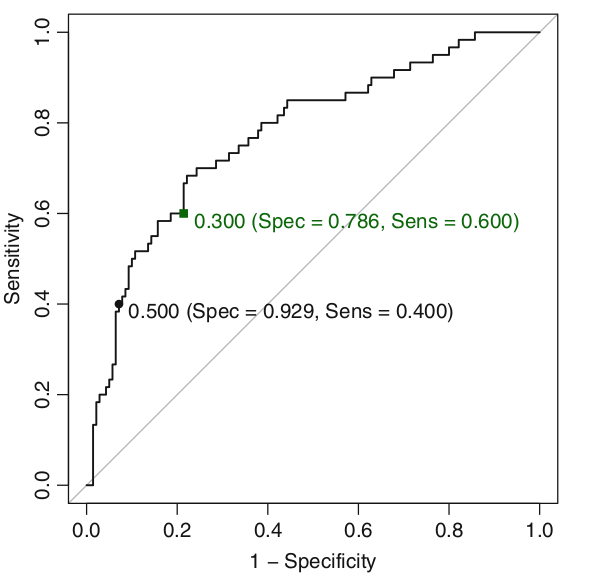
\includegraphics[scale=0.25]{images/ROC curve.png}
\caption{ROC curve of a classifier against random guess}
\end{figure}
\end{frame}

\begin{frame}
\frametitle{Some observations on the ROC curve}
\begin{itemize}
\item The bisector is the ROC curve for the random guessing.
\item A perfect classifier has a ROC curve of the type $y=1$. 
\item We can use the AUC of the ROC curve to select a model. This method is threshold-insensitive and insensitive to disparity in the class proportions (it's a function of sensitivity and specificity).
\item Problems:
\begin{itemize}
\item different curves could cross
\item maybe the threshold is an important discriminating factor.
\item when we will deal with very imbalanced dataset is not reliable.
\end{itemize}
\end{itemize}
\end{frame}

\begin{frame}
\frametitle{Select a threshold using ROC curve}
\begin{itemize}
\item When we are interested in the threshold selection we have to find a trade-off between specificity and sensitivity.
\item We can use the \textbf{\textit{Youden's J index}}:
$$
J = Sensitivity + Specificity - 1
$$
and finding the threshold that maximizes this function.
\item Sometimes we can also use this indicator:
$$
I = Sensitivity\cdot Specificity
$$
\end{itemize}
\end{frame}

\begin{frame}
\frametitle{PPV and NPV}
We introduce two other important metrics:
\begin{itemize}
\item Positive Predicted Value (or precision) definied as:
$$
\mbox{PPV} = \dfrac{\# \mbox{positive samples and predicted to be positives}}{\# \mbox{Samples predicted as positive}} = \dfrac{\mbox{TP}}{\mbox{TP + FP}}
$$
\item Negative Predicted Value definied as:
$$
\mbox{NPV} = \dfrac{\# \mbox{negative samples and predicted to be negative}}{\# \mbox{Samples predicted as negative}} = \dfrac{\mbox{TN}}{\mbox{TN + FN}}
$$
\item With the PPV and NPV we are seeing how a prediction is reliable.
\end{itemize}
\end{frame}

\begin{frame}
\frametitle{An example of PPV and NPV computation}
Let's suppose we have a confusion matrix like that:
\begin{table}
\begin{tabular}{l | c | c | c | c }
Predicted | Reference & Positive & Negative \\
\hline \hline
Positive + & 300 & 60 \\ 
Negative - & 200 & 855 \\
\end{tabular}
\end{table}
In this case the PPV is:
$$
\dfrac{300}{300 + 60}\cdot 100 = 83 \% 
$$
and the NPV is:
$$
\dfrac{855}{855 + 200}\cdot 100 = 83 \% 
$$
\end{frame}

\begin{frame}
\frametitle{Probabilist interpretation}
\begin{itemize}
\item PPV and NPV are two conditional probabilities too.
\item We use a medical explaination:
\begin{itemize}
\item PPV is defined as the probability of the presence of disease given a positive test result, i.e., $$P(\mbox{disease present} | \mbox{positive test}).$$
\item NPV is defined as the probability of the absence of disease given a negative test result, i.e., $$P(\mbox{disease absent}| \mbox{negative test}).$$
\end{itemize}
\item We can find a relationship with Sensitivity and Specificity using the Prevalence. 
\end{itemize}
\end{frame}

\begin{frame}
\frametitle{Understanding the role of prevalence in PPV and NPV}
\begin{itemize}
\item We have seen that Sensitivity and Specificity depends only on the test/algorithm.
\item The PPV and NPV cannot be independent from it.
\item We first see some examples to better understand the idea and we see the mathematical proof of the fact.
\end{itemize}
\end{frame}

\begin{frame}
\frametitle{Prevalence effect example}
We take two medical examples where we use the same test with :
\begin{itemize}
\item $\mbox{Sensitivity} = 90\%$
\item $\mbox{Specificity} = 90\%$
\item 1000 people
\end{itemize}
and we change the prevalence from $0.5\%$ to $20\%$.
\end{frame}

\begin{frame}
\frametitle{$\mbox{Prevalence} = 5\%$}
\begin{itemize}
\item First case: $\mbox{Prevalence} = 5\%$ so we have $50$ positive people and 950 negative ones. So the confusion matrix is:

\begin{table}
\begin{tabular}{l | c | c | c | c }
Predicted | Reference & Disease & No Disease \\
\hline \hline
Test + & 45 & 95 \\ 
Test - & 5 & 855 \\
\end{tabular}
\caption{$\mbox{Prevalence} = 5\%$}
\end{table}
The PPV is:
$$
PPV = \dfrac{45}{140}\cdot100= 32\%
$$
that is very low.

\end{itemize}
\end{frame}

\begin{frame}
\frametitle{$\mbox{Prevalence} = 20\%$}
\begin{itemize}
\item Second case: $\mbox{Prevalence} = 20\%$ so we have $200$ positive people and 800 negative ones. So the confusion matrix is:

\begin{table}
\begin{tabular}{l | c | c | c | c }
Predicted | Reference & Disease & No Disease \\
\hline \hline
Test + & 180 & 80 \\ 
Test - & 20 & 720 \\
\end{tabular}
\caption{$\mbox{Prevalence} = 5\%$}
\end{table}
The PPV is:
$$
PPV = \dfrac{180}{260}\cdot100= 69\%
$$
that is quite good.
\end{itemize}
\end{frame}
\begin{frame}
\frametitle{Observation on the examples}
\begin{itemize}
\item The PPV is dependent on the prevalence.
\item The PPV can change from one population to another and the same test can be useful or not.
\end{itemize}
\end{frame}

\begin{frame}
\frametitle{How PPV, specificity, sensitivity and prevalence are related?}
We know that:
$$
P(\mbox{disease}| \mbox{positive test}) = \dfrac{P(\mbox{positive test} | \mbox{disease}) \cdot P(\mbox{disease})}{P(\mbox{positive test})}
$$
from Bayes theorem and:
$$
P(\mbox{disease}) = \mbox{prevalence}
$$
and 
\begin{align}
& P(\mbox{positive test}) = P(\mbox{positive test} | \mbox{disease})\cdot P(\mbox{disease})\\
&+ P(\mbox{positive test} | \mbox{not disease}) \cdot P(\mbox{not disease}) 
\end{align}
and so we obtain:
$$
\mbox{PPV}= \dfrac{\mbox{Sensitivity}\times \mbox{Prevalence}}{(\mbox{Sensitivity}\times \mbox{Prevalence}) + ((1-\mbox{Specificity})\times (1-\mbox{Prevalence}))}
$$
\end{frame}

\begin{frame}
\frametitle{Some observations on the PPV}
\begin{itemize}
\item The PPV is strongly dependent on the prevalence.
\item This dependence is a problem. It's not easy to have an idea of the prevalence.\\ In a spam classifier we can have troubles because there are more schemes to invent spam.\\
In medecine the prevalence can also change according to the geografical position.\\
\end{itemize}
\end{frame}

\begin{frame}
\frametitle{Precision-Recall Curve}
\begin{itemize}
\item If the prevalence is known and fixed the PPV/precision can be useful.
\item There is a trade-off between precision and recall related to the threshold chosen. If we increase the threshold we increase the precision but decrease the recall.
\vspace{2mm}
\begin{figure}[ht]
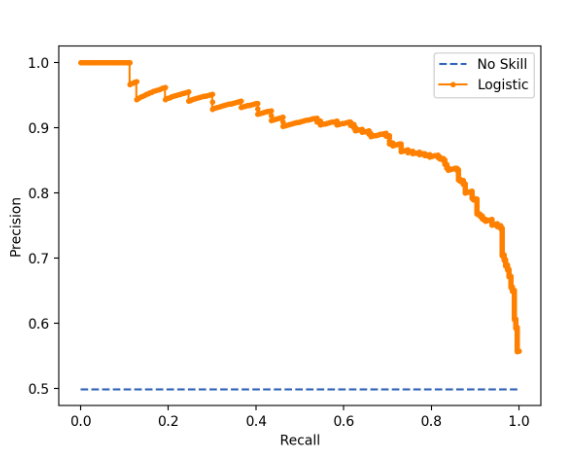
\includegraphics[scale=0.25]{images/precision-recall.png}
\caption{Precision-Recall curve}
\end{figure}
\end{itemize}
\end{frame}

\begin{frame}
\frametitle{Select a threshold using precision-recall curve}
\begin{itemize}
\item When we are interested in the threshold selection we have to find a trade-off between precision and recall.
\item We can use the \textbf{\textit{F1 score}}:
\begin{align}
F_1 = \dfrac{2}{\dfrac{1}{\mbox{precision}} +\dfrac{1}{recall}} = 2\times\dfrac{\mbox{precision} \times \mbox{recall}}{\mbox{precision} + \mbox{recall}}
\end{align}
and finding the threshold that maximizes this function.
\item Sometimes we can also be more interested on precision or more on recall and we don't want to maximize the trade-off. It depends on the situation.
\end{itemize}
\end{frame}

\begin{frame}
\frametitle{What curve is better?}
\begin{itemize}
\item It can be difficoult to chose between the ROC and precision-recall curve to select the best threshold.
\item In a very imbalanced dataset (1:100), if the prevalence is known and constant, it's better to use the precision-recall curve because the ROC is optimistic.
\item This is related to the fact that the false positive rate is:
$$
FPR = 1 - \mbox{Specificity}= \dfrac{FP}{TN + FP}
$$
and $FP$ can be very different in order of magnitude with respect to $TN$. So we can have a $FP$ number high w.r.t. $TP$ but low w.r.t. $TN$. Therefore we can have a very good recall and sensitivity and low precision.
\end{itemize}
\end{frame}

\begin{frame}
\frametitle{Example of ROC problem}
Let's see an example of the previous problem.\\
\begin{table}
\begin{tabular}{l | c | c | c | c }
Predicted | Reference & Negative & Positive \\
\hline \hline
Negative & 9.4e+04 & 10 \\ 
Positive & 4.4e+03 & 1.6e+02 \\
\end{tabular}
\end{table}
In this case we have:
\begin{itemize}
\item Sensitivity: 0.94
\item Specificity: 0.95
\item Precision: 0.035
\end{itemize}
\end{frame}

\begin{frame}{}
\begin{figure}[ht]

\includegraphics[scale=0.25]{images/thankyou.jpeg}
\end{figure}
  \centering \Huge
  \emph{\textbf{Thank you for your attention!!}}
\end{frame}

\end{document}
